%!TEX root = ../thesis.tex
%*******************************************************************************
%****************************** DPD-OSPR Chapter **********************************
%*******************************************************************************
\chapter{Digital Pre-Distorted One-Step Phase Retrieval (DPD-OSPR) Algorithm} \label{chapter:Digital Pre-Distorted One-Step Phase Retrieval (DPD-OSPR) Algorithm}

\graphicspath{{Chapter_DPD_OSPR/Figs/}}

\textit{Note: The work in this chapter has been published in Ref. \cite{Sha2023DPD}}\\\\

In a computer-generated holographic projection system, the image is reconstructed via the diffraction of light from a spatial light modulator. In this process, several factors can contribute to non-linearities between the reconstruction and the target image. This chapter first evaluates the non-linearity of the overall holographic projection system experimentally, using binary phase holograms computed by the OSPR algorithm introduced in \cref{sec:One Step Phase Retrieval (OSPR) Algorithm}. It then applies a digital pre-distortion (DPD) method to correct for the non-linearity. Both a notable increase in reconstruction quality and a significant reduction in mean squared error were observed, which proves the effectiveness of the proposed DPD-OSPR algorithm.


\section{Introduction}
\cref{chapter:Literature Review} reviewed the real-time CGH method called OSPR (in \cref{sec:One Step Phase Retrieval (OSPR) Algorithm}), which was fast enough for real-time holography, but its reconstruction quality can still be potentially improved. Hence, a computationally inexpensive method is needed to improve the reconstruction quality whilst maintaining the real-time property of the OSPR algorithm.

Several factors contribute to the non-linearities between the reconstruction of hologram and the target image, including the calculation and quantisation of the hologram, the modulation of the light and the imperfections in the optical setup. This chapter proposes the digital pre-distorted one-step phase retrieval (DPD-OSPR) algorithm. The digital pre-distortion (DPD) is carried out on the holographic projection system by measuring the non-linearity experimentally and applying the according pre-distortion curve on target images. DPD can be implemented via a one-to-one correction curve or through a look-up table (LUT) which allows the relationship between the input and output to be adjusted without requiring any heavy computation.

The intuition of the proposed DPD-OSPR algorithm for CGH originates from the gamma correction method for conventional displays, such as cathode-ray tube (CRT) monitors \cite{Xu2009}, plasma display panel televisions (PDP-TV) \cite{Sung2009} and thin-film-transistor liquid-crystal displays (TFT LCD) \cite{Lee2005,Prraga2014}. Gamma correction for conventional displays were originally developed to mimic the perceptual response of human vision \cite{Poynton2012}. The work presented here builds logically on this approach and extends its application to holographic displays.



% \section{Method}
% The proposed DPD-OSPR method builds on the OSPR algorithm \cite{Cable2004}, described in \cref{alg:One-Step Phase Retrieval (OSPR) algorithm}, where the propagation function $\mathcal{P}$ is set to Fraunhofer diffraction (in \cref{eq:fraunhofer-diffraction}) and the number of sub-frames $S$ is set to 24 throughout this chapter.

\section{Experimental setup} \label{sec:experimental setup}

\begin{figure}[H]
    \centering
    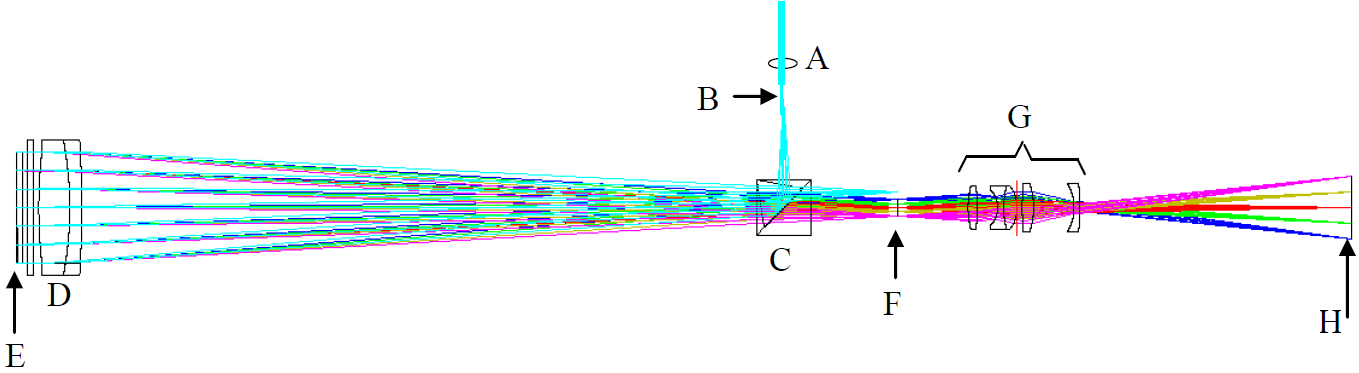
\includegraphics[width=\textwidth]{projection_setup.png}
    \caption{Optical setup of the holographic projection system \cite{Freeman2009}}
    \label{fig:projection_setup}
\end{figure}

The holographic projector used in this experiment is a Fourier projection system developed by Freeman \cite{Freeman2009}, as shown in \cref{fig:projection_setup}. The design is consisted of a diode-pumped solid-state (DPSS) 532 nm 50mW laser source, focussed down by an aspheric singlet (A), the focus of which becomes the diffraction limited point source (B) for the projector. The beam then passes through a polarizing beam splitter cube (C) to a collimating lens (D), which illuminates the SLM (E). The SLM is a binary phase SXGA-R2 ForthDD ferroelectric Liquid crystal on silicon (LCOS) micro-display with a refresh rate of 1440Hz, a pixel pitch of \SI{13.6}{\micro\metre} and a resolution of $1280px \times 1024px$. An aperture at point (F) spatially filters out the other orders, leaving only one first order, which is then magnified up by a finite conjugate lens group (G) to produce an image, of the required size, on the screen (H). \cite{Freeman2009}

\begin{figure}[H]
    \centering
    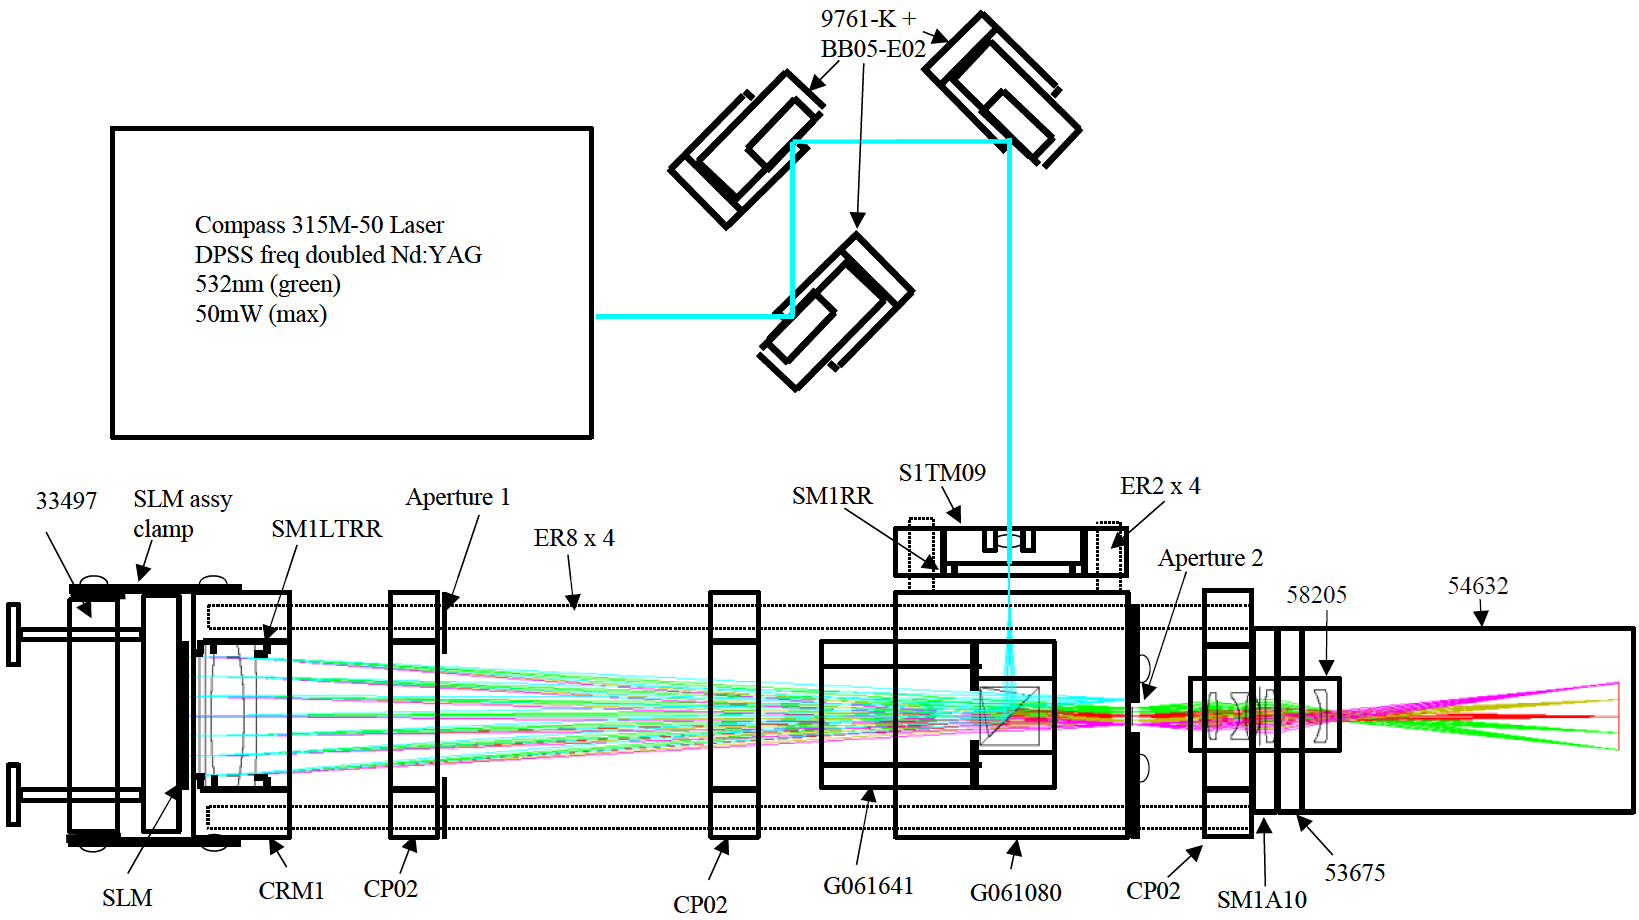
\includegraphics[width=\textwidth]{holographic_projector.png}
    \caption{Mechanical components with part numbers of the holographic projection system \cite{Freeman2009}}
    \label{fig:holographic_projector}
\end{figure}

The mechanical components are listed in \cref{fig:holographic_projector} with part numbers. The holograms displayed on the SLM are generated using the OSPR algorithm \cite{Cable2004}, and as the SLM is a binary-phase modulator, each hologram sub-frame needs to be binary quantised. Then each group of the 24 binary-phase hologram sub-frames are encoded as the 8-bit red, green, blue (RGB) channels of a 24-bit image to interface with the SLM driver electronics. The SLM displays each bit plane sequentially, with ones and zeros mapping to opposing phase modulations at each pixel. The reconstructions were captured using a Canon 550D camera with an EFS 18-55 mm lens. To ensure fair comparison, the camera was set to the same manual setting when comparing each pair of replay fields before and after DPD. It takes $24/1440=1/60$s to display all 24 sub-frames on a 1440Hz SLM, so the camera shutter speed was set to $1/30$s to capture all frames twice. The images captured are raw format in RGB colour, which are subsequently converted to grey-scale (using the rgb2gray function in Matlab\cite{MATLAB}) when calculating NMSE against the target images, using the equation $NMSE = \frac{\frac{1}{n} * \sum (x - \hat{x})^2}{\sum (x)^2}$, where $x$ is the target, $\hat{x}$ is the measured output and $n$ is the dimension of $x$ and $\hat{x}$.



\section{Determining the DPD curve}

\begin{figure}[H]
    \centering
    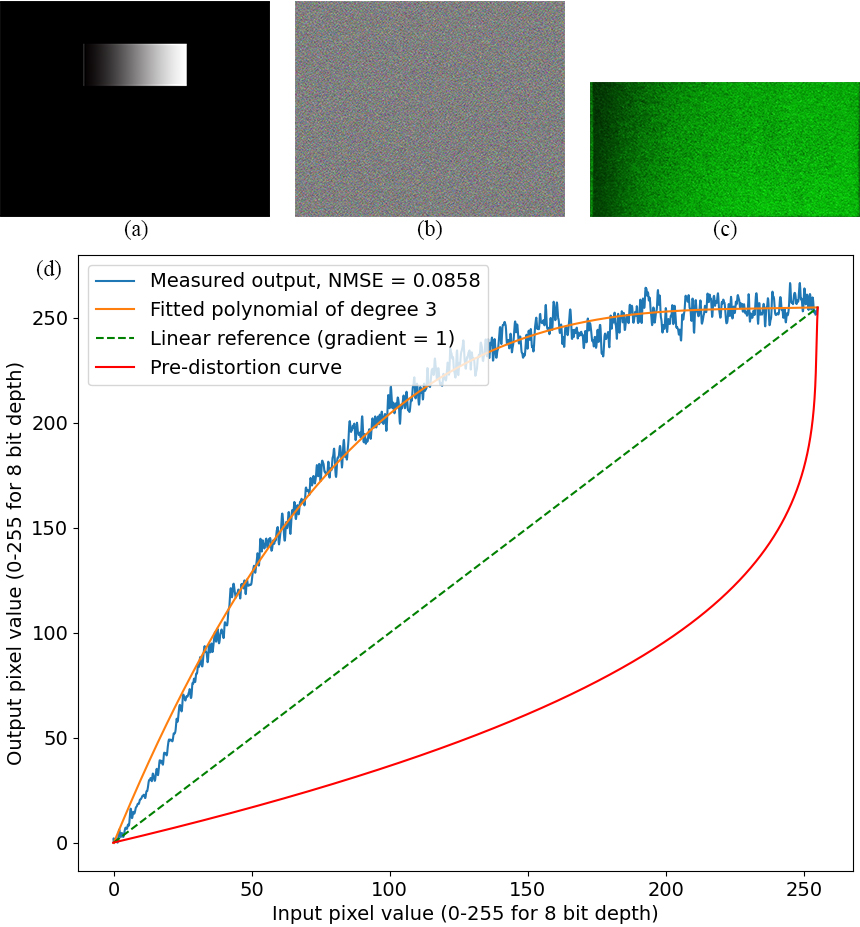
\includegraphics[width=\textwidth]{Determining_the_DPD_curve.jpg}
    \caption{Determining the DPD curve. (a) Input linear grey-scale ramp. (b) Corresponding CGH of (a) with 24-subframe binary phase encoding. (c) Holographic projection replay field of (b). (d) Plot of non-linearity measurement and according pre-distortion curve.}
    \label{fig:Determining_the_DPD_curve}
\end{figure}

To determine the DPD curve of the holographic projection system, the non-linearity needs to be measured first. The hologram in \cref{fig:Determining_the_DPD_curve}(b) was first generated using OSPR algorithm for the linear grey-scale ramp of pixel value increasing linearly from 0 to 255, as shown in \cref{fig:Determining_the_DPD_curve}(a), along with a single pixel white (255) strip at the left end as a fiducial marker to demonstrate the beginning of the grey-scale region \cite{Cable2006}.

The projection output of the linear grey-scale ramp was then captured and cropped as shown in \cref{fig:Determining_the_DPD_curve}(c), from which the non-linearity curve was determined, by averaging each column of pixels in the image and discarding the fiducial marker, forming the blue line in \cref{fig:Determining_the_DPD_curve}(d). A third-order polynomial fit was applied, generating a smoothed non-linearity curve (yellow line in \cref{fig:Determining_the_DPD_curve}(d)).

There exhibits a high degree of non-linearity. By taking the mean of the square of the error between the measured output (blue line) and the linear reference (green dashed line), the normalized mean squared error (NMSE) of the measured output was calculated to be 0.0858. To correct for the non-linearity, the DPD curve (red line) was formed by inverting the smoothed non-linearity curve (yellow line) in \cref{fig:Determining_the_DPD_curve}(d).

\begin{figure}[H]
    \centering
    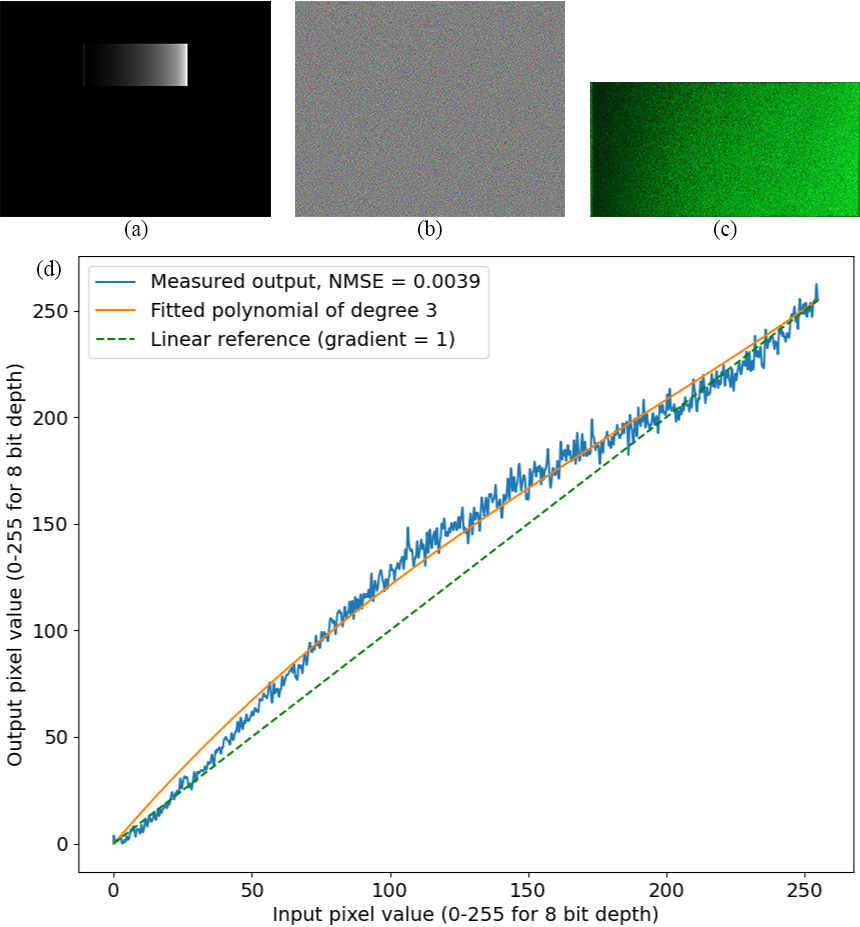
\includegraphics[width=\textwidth]{Validation_of_DPD_curve_on_the_grey-scale_ramp.jpg}
    \caption{Validation of DPD curve on the grey-scale ramp. (a) Pre-distorted ramp. (b) Corresponding CGH of (a) with 24-subframe binary phase encoding. (c) Holographic projection replay field of (b). (d) Non-linearity measurement after DPD.}
    \label{fig:Validation of DPD curve on the grey-scale ramp}
\end{figure}
\vspace{3mm}

Subsequently, the DPD curve (red line in \cref{fig:Determining_the_DPD_curve}(d)) was used to adjust the grey-scale ramp, achieving the pre-distorted grey-scale ramp as shown in \cref{fig:Validation of DPD curve on the grey-scale ramp}(a). The according projection output was then captured as shown in \cref{fig:Validation of DPD curve on the grey-scale ramp}(c). By using the same method of averaging columns of pixels, the measured output was plotted in \cref{fig:Validation of DPD curve on the grey-scale ramp}(d). It can be seen that the corrected non-linearity was much closer to linear comparing to the original non-linearity, and the NMSE was calculated to be 0.0039.

\begin{table}[H]
    \begin{center}
        \begin{tabular}{|c|c|c|}
            \hline
                       & NMSE   & Percentage \\ \hline
            Before DPD & 0.0858 & 100\%      \\ \hline
            After DPD  & 0.0039 & 4.55\%     \\ \hline
        \end{tabular}
        \caption{Non-linearity results before and after DPD}
        \label{tab:non-linearity result}
    \end{center}
\end{table}

Hence, as demonstrated in \cref{tab:non-linearity result}, DPD achieved a 95.45\% reduction in NMSE, which was a significant improvement in non-linearity, therefore the DPD curve measured is validated.




\section{Applying the DPD Curve}

\begin{figure}[H]
    \centering
    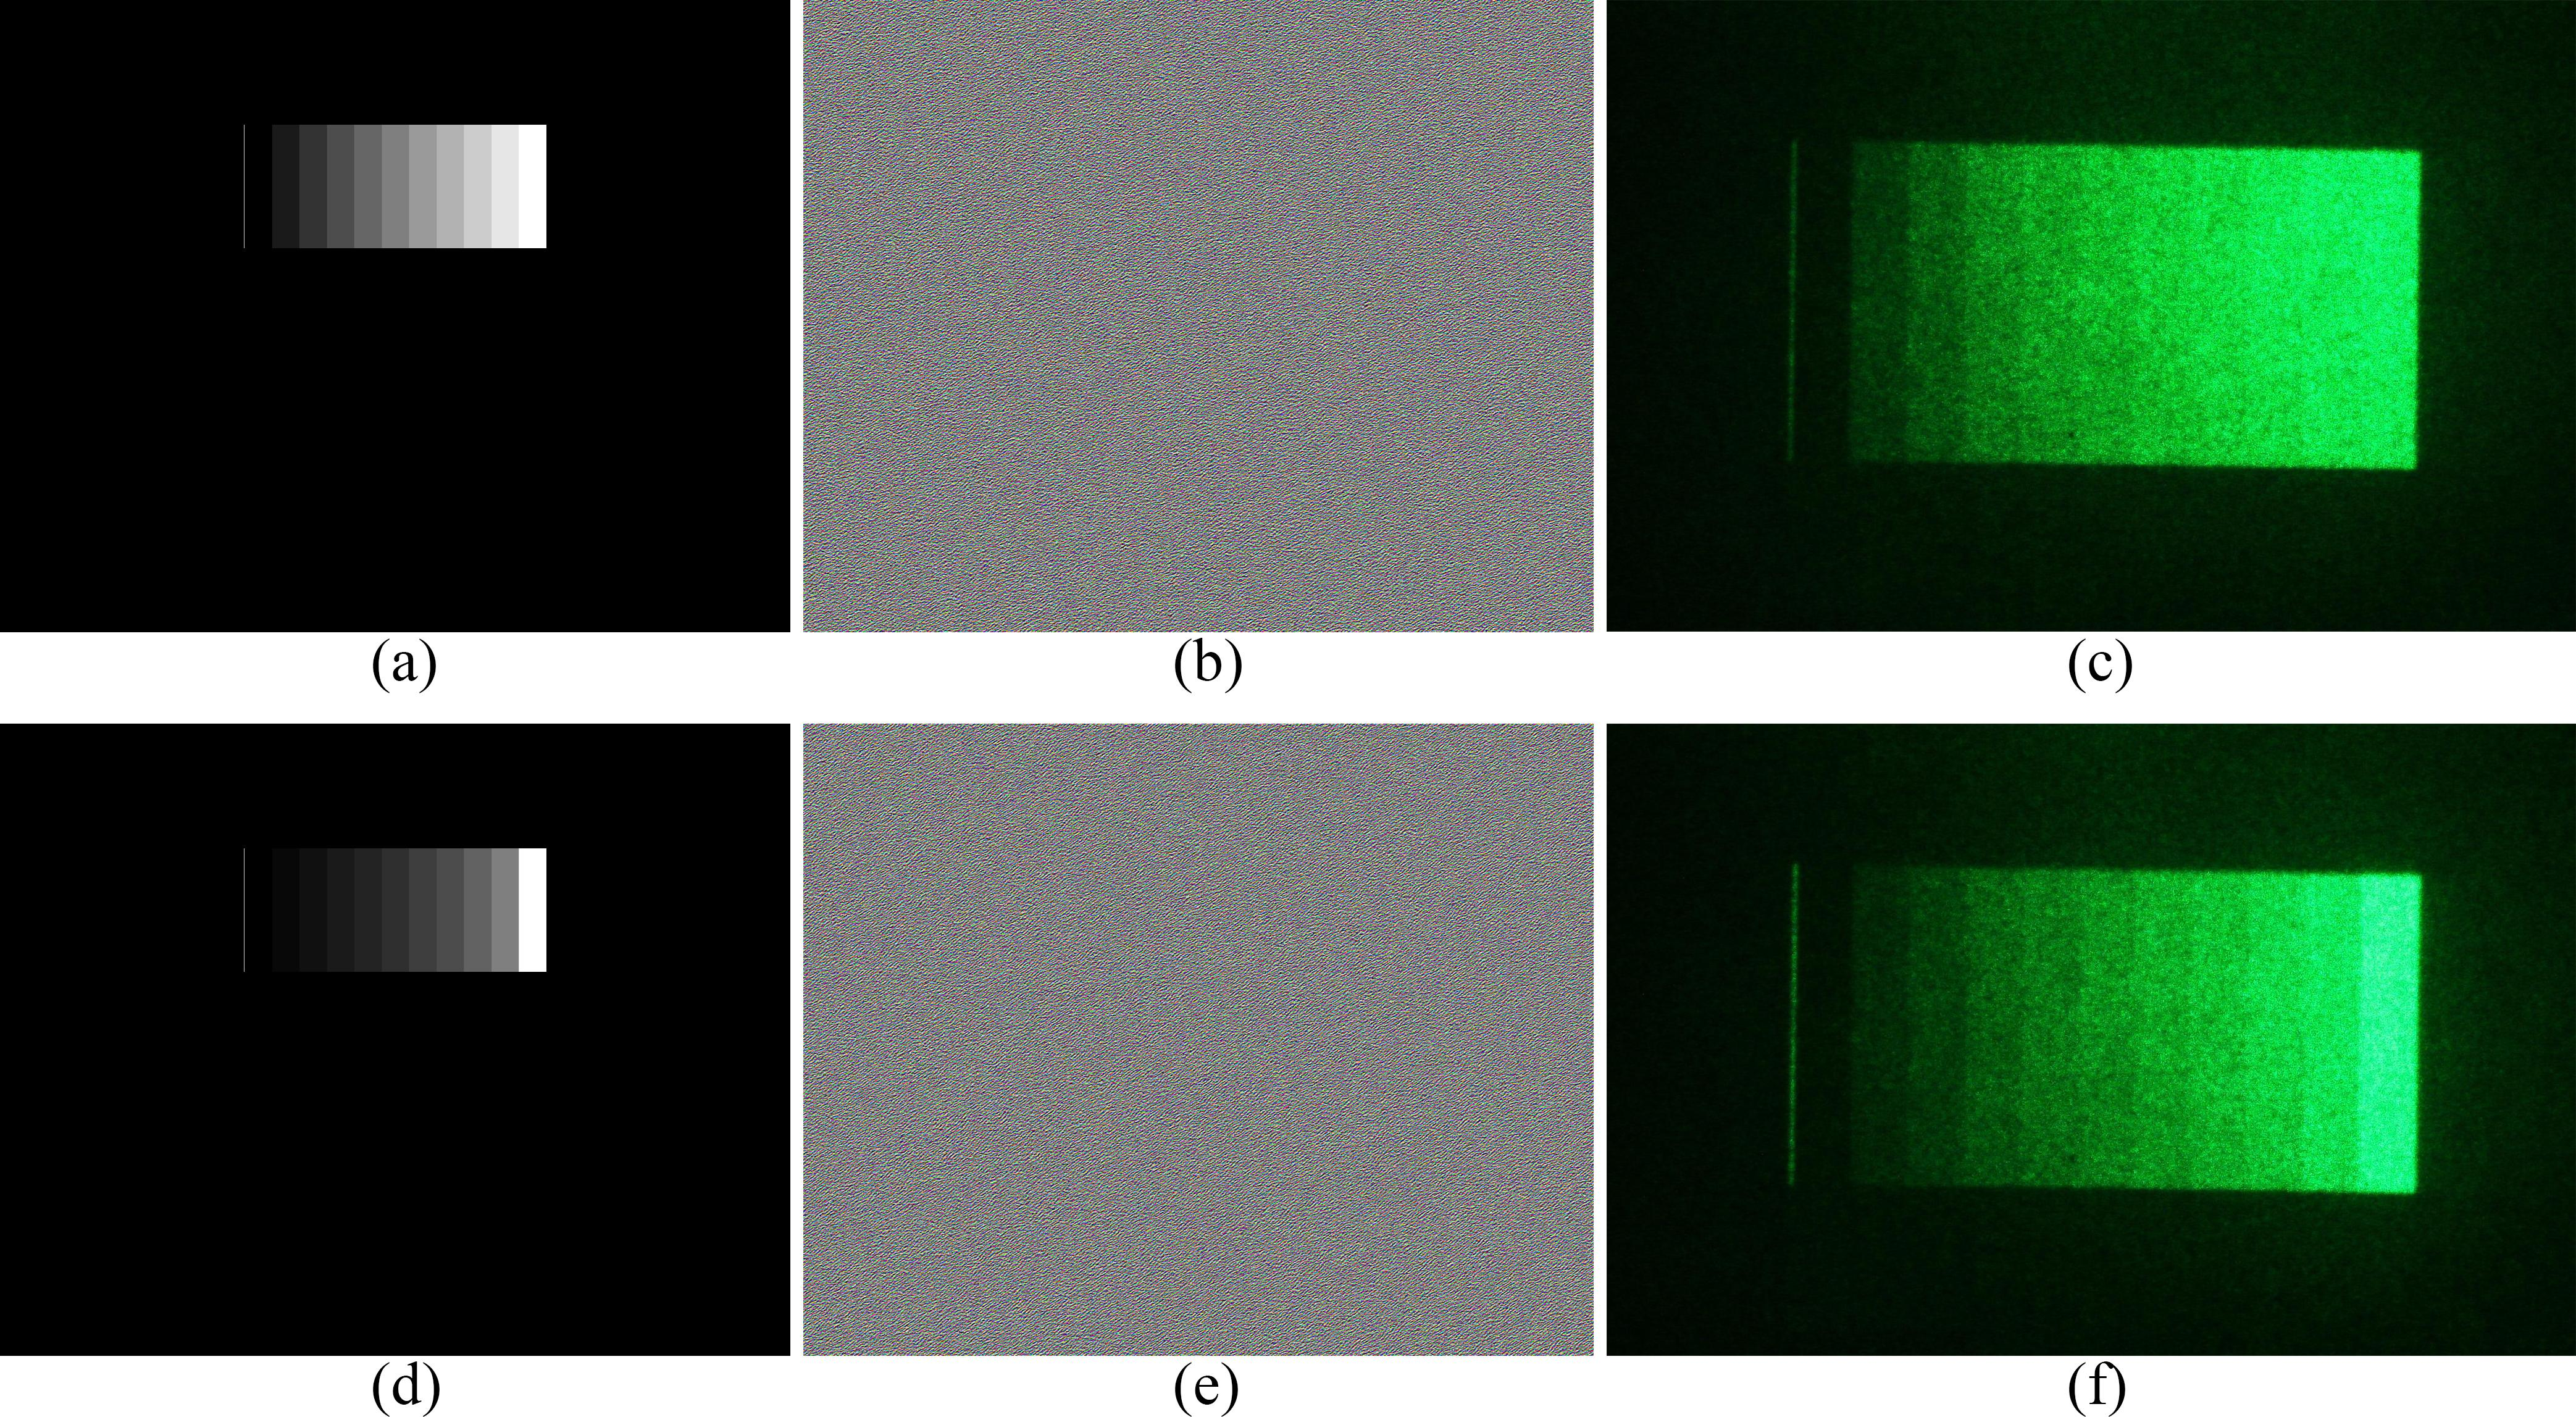
\includegraphics[width=\textwidth]{10_step_strips.jpg}
    \caption{Application of DPD on the 10-step strips. (a) 10 strips with equal step of pixel value. (b) CGH of (a). (c) Holographic projection replay field of (b). (d) After DPD of (a). (e) CGH of (d). (f) Holographic projection replay field of (e).}
    \label{fig:10_step_strips}
\end{figure}
\vspace{3mm}

To qualitatively demonstrate the effectiveness of our approach, we project a simple test pattern of a graduated ramp test pattern consisted of 10-step strips in \cref{fig:10_step_strips}(a), which is commonly employed in gamma-correction calibration of many display systems. As shown in the projection replay field captured in \cref{fig:10_step_strips}(c), before DPD, the right few strips are barely distinguishable. In comparison, after carrying out DPD, it can be seen that each pair of adjacent strips in \cref{fig:10_step_strips}(f) are much more distinguishable, qualitatively showing the effectiveness of the DPD method.

\begin{figure}[H]
    \centering
    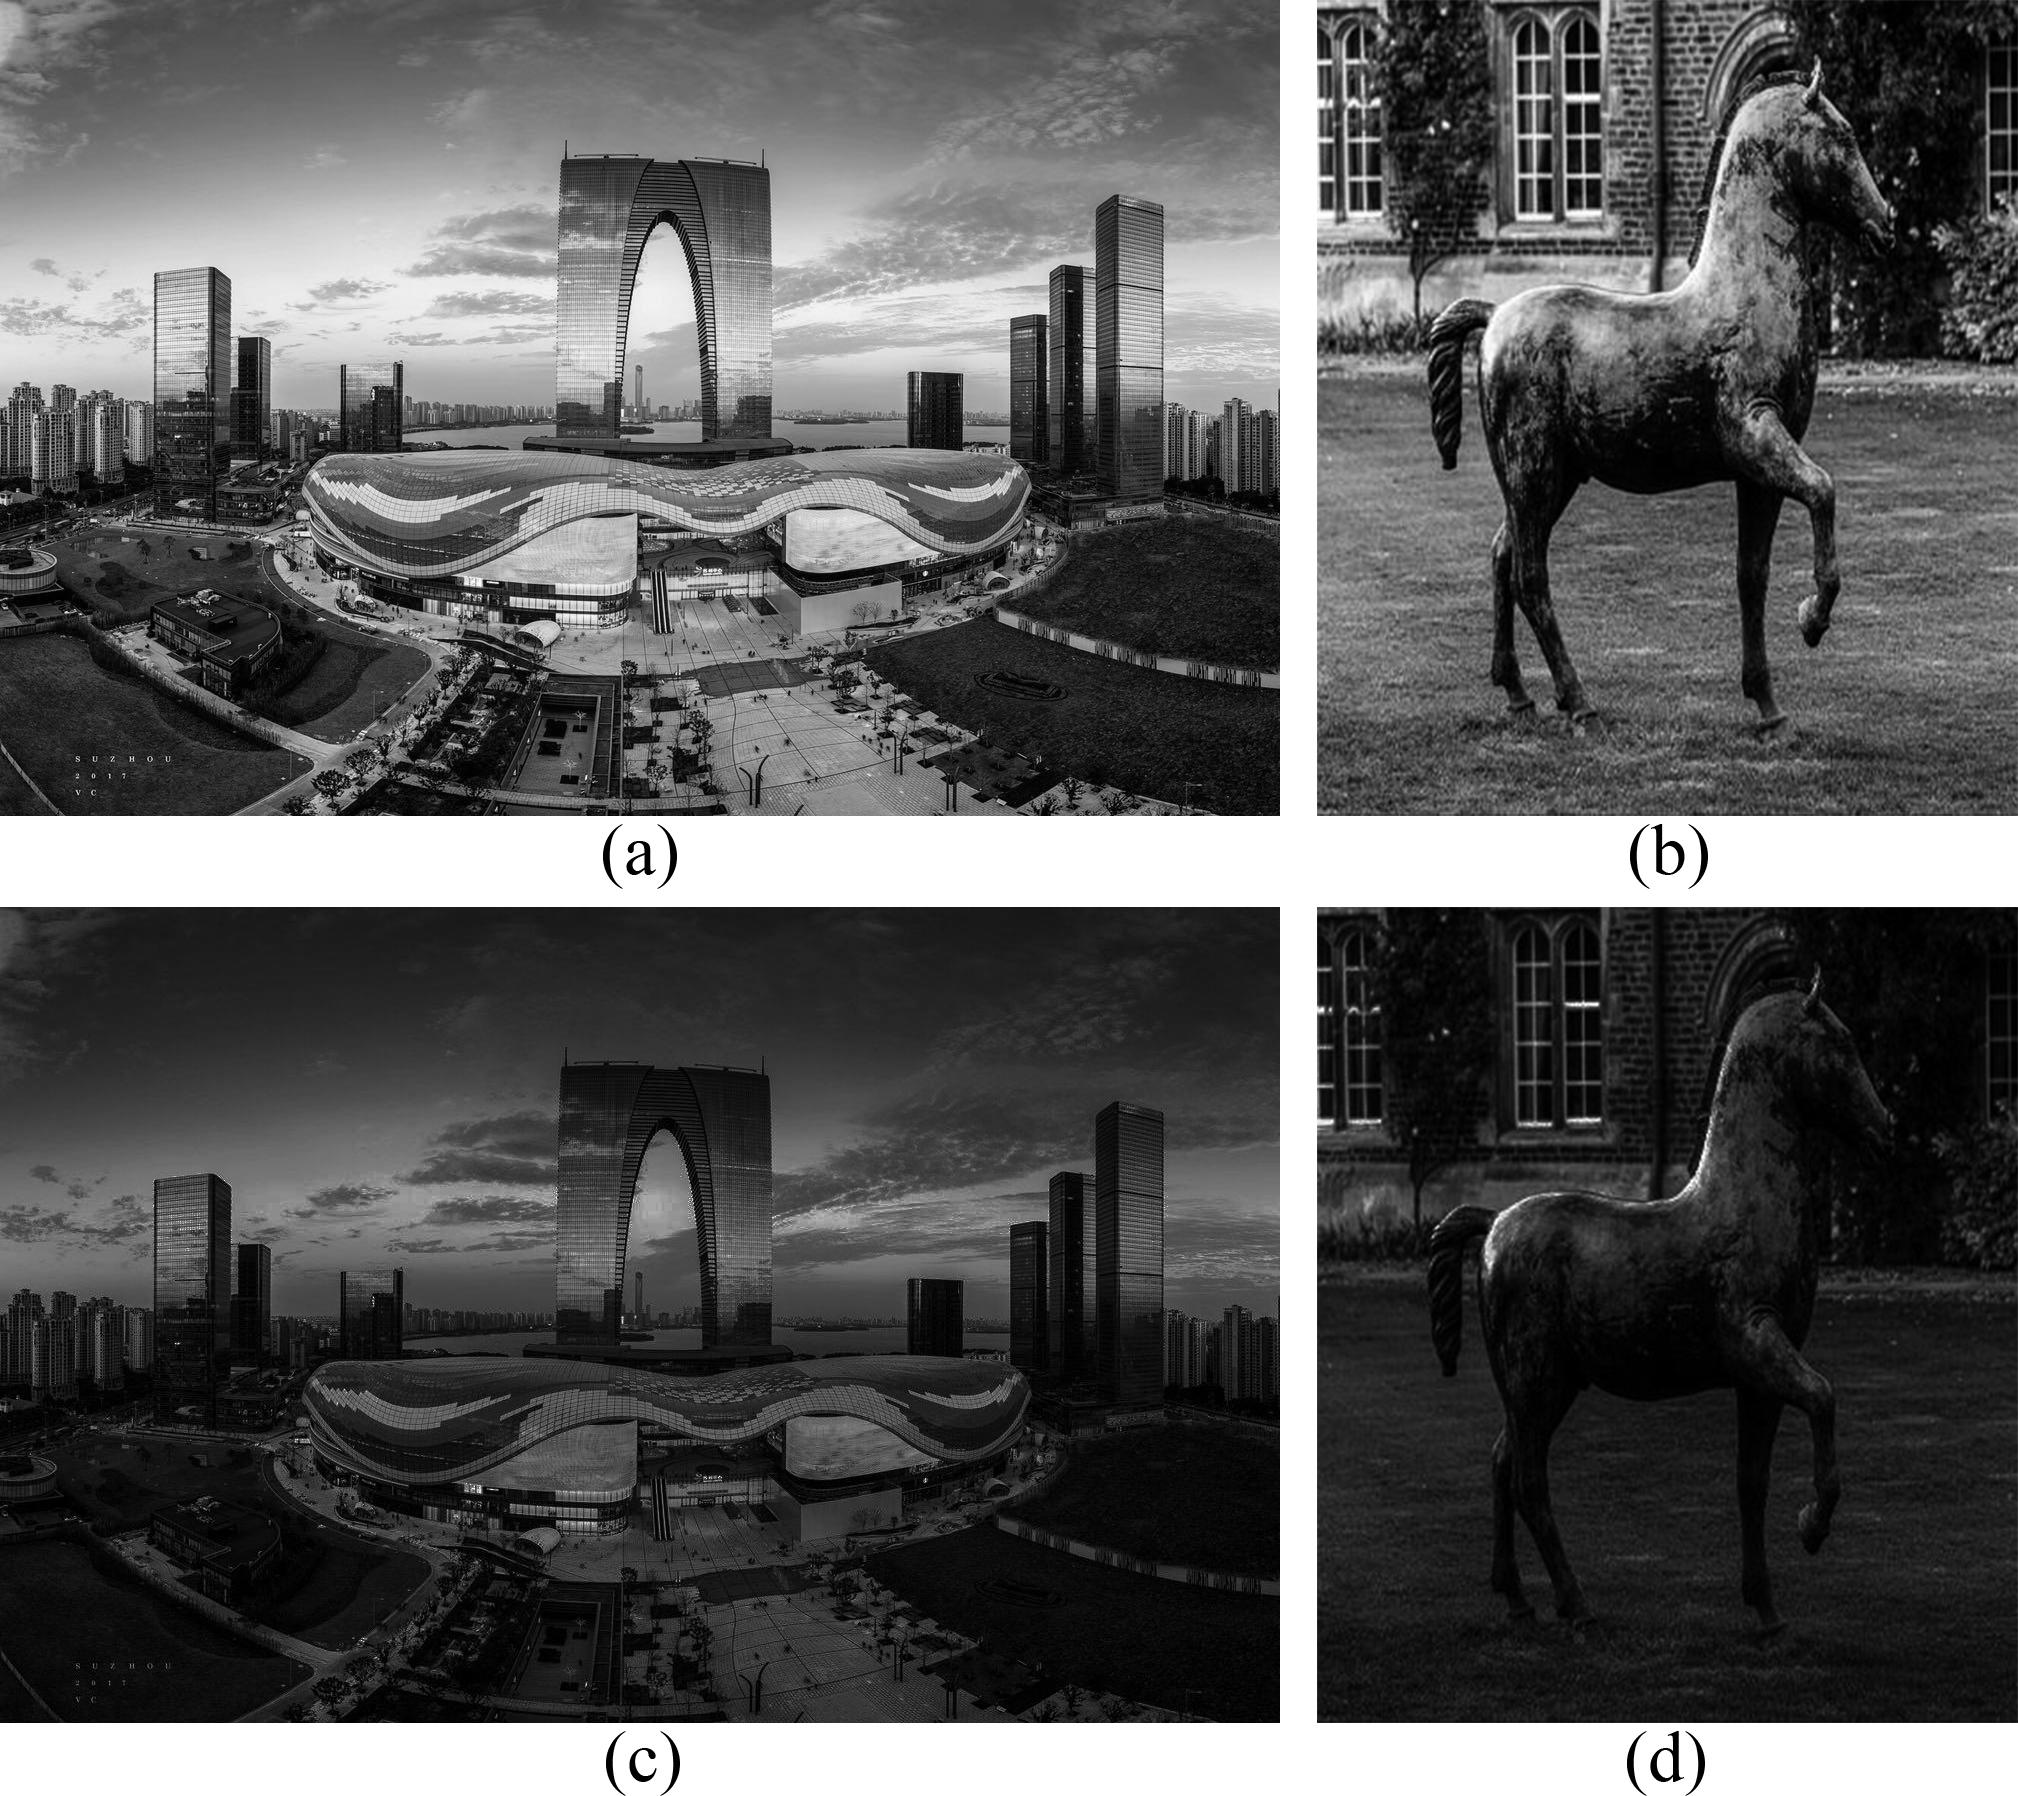
\includegraphics[width=\textwidth]{Application_of_DPD_on_two_sample_real-word_images.jpg}
    \caption{Application of DPD on two sample real-word images. (a) Sample image 1: City Scene \cite{Zhao2017}. (b) Sample image 2: Horse. (c) Sample image 1 after DPD. (d) Sample image 2 after DPD.}
    \label{fig:Application of DPD on two sample real-word image}
\end{figure}
\vspace{3mm}

Then the DPD curve was applied to the two sample images as shown in \cref{fig:Application of DPD on two sample real-word image} (a) and (b), producing pre-distorted images in \cref{fig:Application of DPD on two sample real-word image} (c) and (d). Holograms were generated for each image using the OSPR algorithm and loaded onto the SLM respectively. The according replay fields were captured as shown in \cref{fig:Projection output of the two sample images before and after DPD}.

\begin{figure}[H]
    \centering
    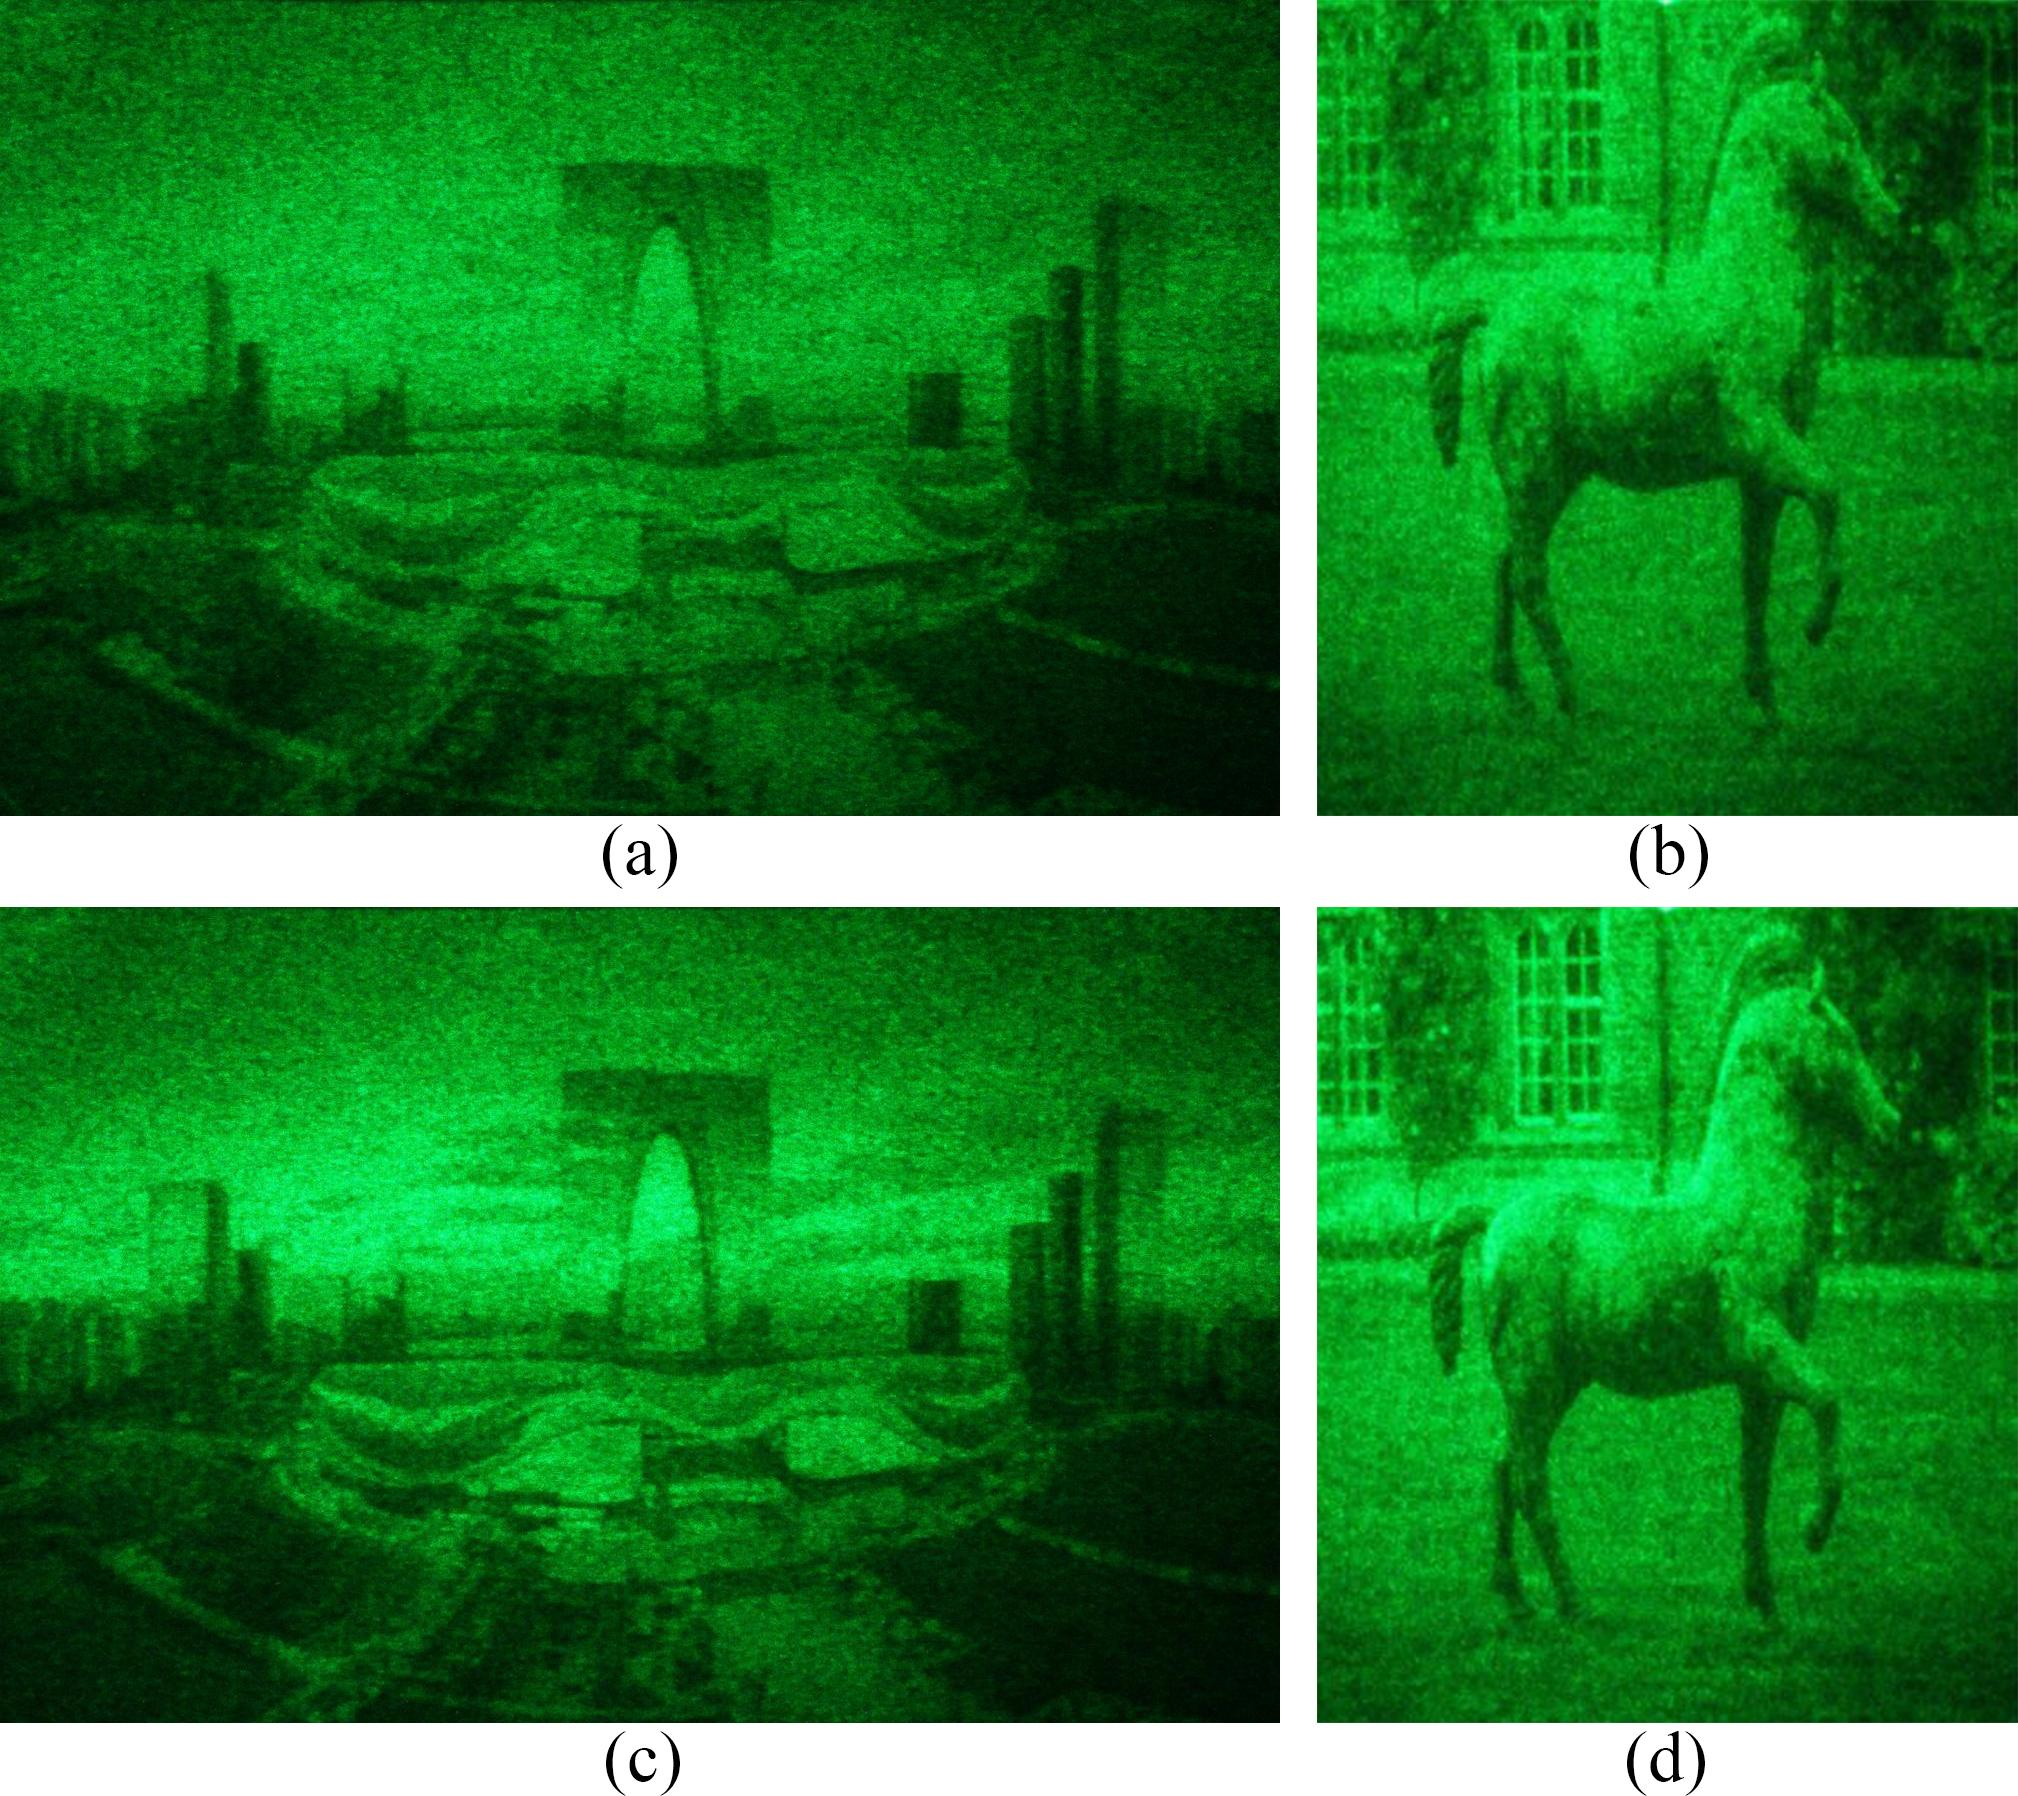
\includegraphics[width=\textwidth]{Projection_output_of_the_two_sample_images_before_and_after_DPD.jpg}
    \caption{Projection output of the two sample images before and after DPD. (a) Replay field of Sample image 1 before DPD (NMSE=0.06139). (b) Replay field of Sample image 2 before DPD (NMSE=0.04309). (c) Replay field of Sample image 1 after DPD (NMSE=0.04920). (d) Replay field of Sample image 2 after DPD (NMSE=0.03635).}
    \label{fig:Projection output of the two sample images before and after DPD}
\end{figure}
\vspace{3mm}

The replay fields of the holographic projection of original images are shown in \cref{fig:Projection output of the two sample images before and after DPD} (a) and (b), and the replay fields of the holographic projection of images after DPD are shown in \cref{fig:Projection output of the two sample images before and after DPD} (c) and (d).

As shown in \cref{fig:Projection output of the two sample images before and after DPD}(a), it can be seen that, before DPD, the edges between the buildings and the sky were quite ambiguous, with most detail of the sky being lost. In comparison, after DPD, the replay field in \cref{fig:Projection output of the two sample images before and after DPD}(c) provided not only sharper edges between buildings and the sky, but also more detail of clouds in the sky. The NMSE of the replay field for sample image 1 decreased from 0.06139 to 0.04920, which was a 19.86\% reduction.

In \cref{fig:Projection output of the two sample images before and after DPD}(b), before DPD, the horse was difficult to distinguish from the background, especially around the horse's back area. But after DPD, as shown in \cref{fig:Projection output of the two sample images before and after DPD}(d), contrast has been significantly boosted and the fine detail around this part of the horse is more evident. The NMSE of the replay field for sample image 2 decreased from 0.04309 to 0.03635, which was a 15.64\% reduction.


\begin{table}[H]
    \begin{center}
        \begin{tabular}{ccc}
            \hline
            \multicolumn{1}{|c|}{Sample image 1} & \multicolumn{1}{c|}{NMSE}    & \multicolumn{1}{c|}{Percentage} \\ \hline
            \multicolumn{1}{|c|}{Before DPD}     & \multicolumn{1}{c|}{0.06139} & \multicolumn{1}{c|}{100\%}      \\ \hline
            \multicolumn{1}{|c|}{After DPD}      & \multicolumn{1}{c|}{0.04920} & \multicolumn{1}{c|}{80.15\%}    \\ \hline\hline
            \multicolumn{1}{|c|}{Sample image 2} & \multicolumn{1}{c|}{NMSE}     & \multicolumn{1}{c|}{Percentage} \\ \hline
            \multicolumn{1}{|c|}{Before DPD}     & \multicolumn{1}{c|}{0.04309} & \multicolumn{1}{c|}{100\%}      \\ \hline
            \multicolumn{1}{|c|}{After DPD}      & \multicolumn{1}{c|}{0.03635} & \multicolumn{1}{c|}{84.36\%}    \\ \hline
        \end{tabular}
        \caption{DPD results for sample images}
        \label{tab:DPD results for sample images}
    \end{center}
\end{table}

Hence, as summarised in \cref{tab:DPD results for sample images}, DPD achieved a 19.86\% reduction in NMSE for sample image 1 and a 15.64\% reduction in NMSE for sample image 2, quantitatively proving the effectiveness of DPD method for CGH of real-world test images using OSPR algorithm.

Lastly, as the DPD is a one-to-one mapping, the computation time is negligible. In practice, the computational overhead is too small to be measured against randomness between subsequent runs. DPD can also be further accelerated in hardware using a hardware LUT, so that the DPD can be carried out instantly. This approach is widely adopted in gamma correction for displays.




\section{Summary}
The non-linearity between the target image and the reconstructed image was measured for the overall holographic projection system by projecting a linear grey-scale ramp. The DPD curve was then applied to the grey-scale ramp, successfully reducing the NMSE by 95.45\%. To evaluate its effectiveness on real world images, the DPD method was applied on two sample images. It was observed that more details were shown in the replay field after DPD, and the NMSE's of the two example images were reduced by 19.86\% and 15.64\%, respectively. As the DPD is a one-to-one mapping, the extra computation required is negligible. Hence, we have demonstrated the effectiveness of the proposed DPD-OSPR method in improving reconstruction quality over the original OSPR algorithm while still maintaining its capability for real-time holography. The proposed DPD method needs to be applied only once for every holographic projector; however, compared to the original OSPR method, the proposed DPD-OSPR method requires an additional device of a camera, whose accuracy and linearity can adversely affect the effectiveness of the DPD process.
